\frame{
    \frametitle{$\kappa_{2V}$, $\kappa_\lambda$,$\kappa_V$ Linear Combination Scan (Work in Progress...)}
    \begin{columns}
        \begin{column}{0.6\textwidth}
            Linear Combination Equation
            ({\small Based on a pseudo-randomly chosen basis set}):
            \vspace{10mm}

            {\tiny $
A_{0} \left(- 2 \kappa_{2V}^{2} + 6 \kappa_{2V} \kappa_{V}^{2} - 3 \kappa_{2V} \kappa_{V} \kappa_{\lambda} - 4 \kappa_{V}^{4} + 5 \kappa_{V}^{3} \kappa_{\lambda} - \kappa_{V}^{2} \kappa_{\lambda}^{2}\right) + A_{1} \left(- \frac{3 \kappa_{2V} \kappa_{V}^{2}}{2} + \frac{3 \kappa_{2V} \kappa_{V} \kappa_{\lambda}}{2} + \frac{5 \kappa_{V}^{4}}{2} - 3 \kappa_{V}^{3} \kappa_{\lambda} + \frac{\kappa_{V}^{2} \kappa_{\lambda}^{2}}{2}\right) + A_{2} \left(\frac{2 \kappa_{2V}^{2}}{3} - \frac{11 \kappa_{2V} \kappa_{V}^{2}}{6} + \frac{\kappa_{2V} \kappa_{V} \kappa_{\lambda}}{6} + \frac{7 \kappa_{V}^{4}}{6} - \frac{\kappa_{V}^{3} \kappa_{\lambda}}{6}\right) + A_{3} \left(\frac{4 \kappa_{2V}^{2}}{3} - \frac{8 \kappa_{2V} \kappa_{V}^{2}}{3} + \frac{4 \kappa_{2V} \kappa_{V} \kappa_{\lambda}}{3} + \frac{4 \kappa_{V}^{4}}{3} - \frac{4 \kappa_{V}^{3} \kappa_{\lambda}}{3}\right) + A_{4} \left(- \frac{\kappa_{2V} \kappa_{V}^{2}}{2} + \frac{\kappa_{2V} \kappa_{V} \kappa_{\lambda}}{2} + \frac{\kappa_{V}^{4}}{2} - \kappa_{V}^{3} \kappa_{\lambda} + \frac{\kappa_{V}^{2} \kappa_{\lambda}^{2}}{2}\right) + A_{5} \left(\frac{\kappa_{2V} \kappa_{V}^{2}}{2} - \frac{\kappa_{2V} \kappa_{V} \kappa_{\lambda}}{2} - \frac{\kappa_{V}^{4}}{2} + \frac{\kappa_{V}^{3} \kappa_{\lambda}}{2}\right)
$
}
        \end{column}
        \begin{column}{0.4\textwidth}
            \begin{center} \resizebox{0.2\textheight}{!}{\begin{tabular}{ |l|l|l| }
                \hline
                \textbf {$\kappa_{2V}$} & \textbf {$\kappa_\lambda$} & \textbf {$\kappa_V$} \\
                \hline
                1   &  1 &   1 \\
                1   &  0 &  -1 \\
                0   &  1 &   1 \\
                1.5 &  1 &   1 \\
                1   &  2 &   1 \\
                2   &  1 &  -1 \\
                \hline
            \end{tabular}} \end{center}
            \vspace{5mm}
            \begin{figure}
                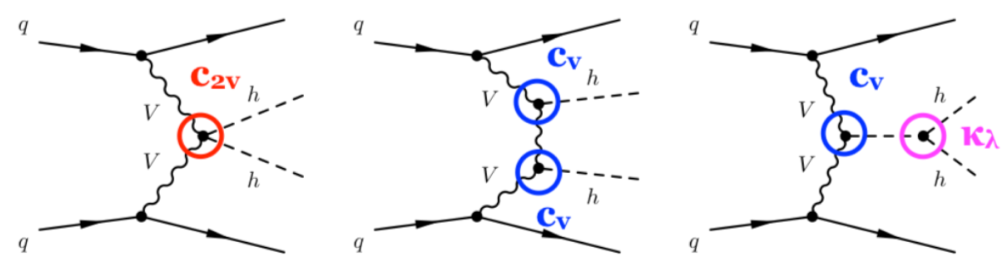
\includegraphics[width=\linewidth,height=\textheight,keepaspectratio]{vbf-hh_diagrams2}
            \end{figure}
        \end{column}
    \end{columns}
}

\displaythree{Comparing Linear Combination with Generated Sample}{
    {\tiny The linear combination successfully fits separately generated MC samples,
    but shows significant deviations that could be corrected with a properly chosen basis set.}
}{mHH_cvv0p5cl1p0cv1p0}
{mHH_cvv2p0cl1p0cv1p0}
{mHH_cvv0p0cl0p0cv1p0}
